

\subsection{Digital Twin and Industry 4.0}
Digital Twin is an integrated software solution with modelling, analytical capability, and interconnectivity technology to replicate the physical world in digital space. The inception of this concept can be traced back to NASA's work on the Apollo 13 space project in 1970, where it was used as 'mirror systems' to troubleshoot and resolve issues \cite{adrienbacueDigitalTwinsEnhanced2022}. However, it was in 2002, the term "Digital Twin" coined for the first time by Michael Grieves and John Vickers of NASA in 2003, specifically for the application of product life cycle management \cite{jones_characterising_2020}.

The concept and definition of Digital Twins have been open to various interpretations, depending on the specific context.  However, through our systematic literature review in chapter \ref{Chapter2}, we identified Digital Twins typically revolve around three fundamental components: \textbf{states} (physical and digital), \textbf{interconnectivity} (communication channel between the physical and virtual state) and \textbf{process} (a mechanism for processing and analysing data). 

\begin{figure}[H]
    \centering
    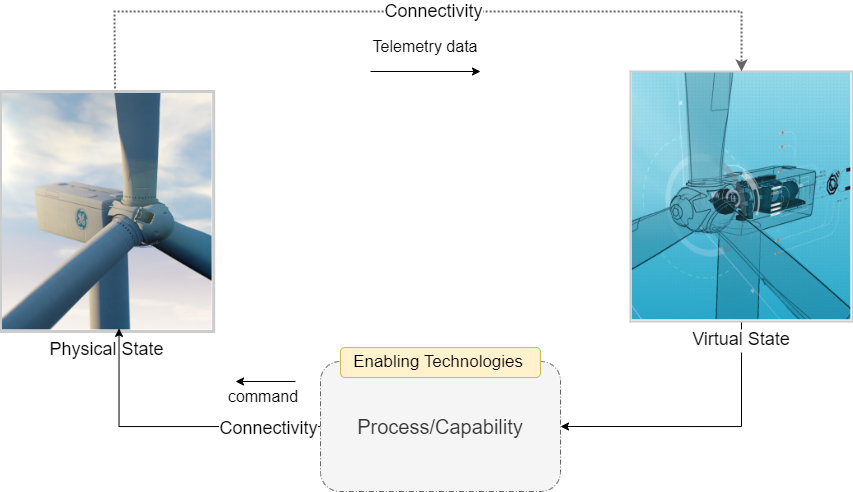
\includegraphics[width=1\linewidth]{images/fp/digital-twin-concept.drawio.png}
    \caption{Three Component of Digital Twin--State, Connectivity, and Capability(Process)}
    \label{fig:dt-concept}
\end{figure}

% Here, we provide a comprehensive definition of Digital Twin synthesised from a collection of various definitions of research publications:

% \textit{ Digital Twin is a virtual representation of a physical object, process or system that mirrors its real-world counterpart through real-time updates and tracking of its entire life-cycle. It is designed to model the physical characteristics and behaviours of the object using digital technology, mapping the physical operating environment to virtual space for interaction, and providing valuable insights through collecting asset-centric data, analytic capabilities, and simulations. Digital twins are used to monitor, simulate, optimise and predict the state of a physical object. They have a standard structure, end-to-end connectivity, communication protocol with backward compatibility, and a standard data format for communication between the twins.}

% The definition and respective reference are listed in Table \ref{tbl:dtconcept}


\begin{itemize}
% Virtual replica, Model, Evolving digital profile 
% A process, product, system, environment, industrial assest 
    \item \textbf{State}: Digit Twin has two states (see \ref{fig:dt-concept}); Virtual and Physical state. The virtual state is a digital (software) replica or model representation of a physical object, closely resembling the physical aspect. It can also be described as an evolving digital profile that captures the historical and current status of the represented object \cite{becueCyberFactorySecuringIndustry40with2018}. The physical state, on the other hand, refers to the real-world object of what the Digital Twin represents. The object that is represented by the virtual state could be physical components, processes \cite{wangDTCPNDigitalTwin2022, sousaELEGANTSecurityCritical2021, lopezDIGITALTWINSINTELLIGENT2021, rebecchiDigitalTwin5G2022, luongnguyenDigitalTwinIoT2022}, products, industrial assets \cite{dietzIntegratingDigitalTwin2020, eckhartEnhancingCyberSituational2019}, and environments.

    \item \textbf{Connectivity}: To keep the virtual state with the physical counterpart, a wired or wireless communication channel must be established. To keep the virtual state fidelity, the physical state should send  telemetry data (environmental sensor measurements) in real time. In this regard, wide sensor arrays can be deployed in the physical world to keep the data flow synchronized \cite{danilczykSmartGridAnomaly2021}. On the other hand, a command (a control message) can be sent from the virtual state to the physical state. Furthermore, ensuring a communication protocol that supports backward compatibility and adheres to a standard data format is required for achieving seamless data exchange between the two states \cite{atalayDigitalTwinsApproach2020}.

 
    \item \textbf{Process/Capability}: The true power of Digital Twin lies primarily due to the utilization of enabling technologies\cite{sousaELEGANTSecurityCritical2021}. This aspect also differentiates Digital Twin from simulation software. The use of enabling technology such as machine learning, blockchain, cloud computing, and big data analytics equipped Digital Twin with capabilities for better decision-making and to be used as a security tool. 
    
    Digital Twin can be equipped with enabling technology to provide various security services. For example,  detecting abnormal process events or deliberately injected malicious content \cite{saadImplementationIoTBasedDigital2020}, for prompt intervention and resolution of issues \cite{akbarianSecurityFrameworkDigital2021}, as a cyber situational awareness tool \cite{eckhartEnhancingCyberSituational2019} and so on.  
    
% In most definitions, Digital Twin is intended for simulation. One definition elaborates the simulation function as an insight gained through collecting asset-centric data. In quite a number of definitions, it is also stated that the digital twin is used for monitoring and controlling the real-world counterparts. In one definition the authors argued it can be used to increase cyber situational awareness for Cyber Critical Infrastructures


% In conclusion, Of the three core components of Digital Twin, only the "state" is explicitly described within the definition. The intended purpose and the interconnectivity between the two states are not always included in the provided definition.


    
\end{itemize}


% \begin{table}[H]
% \small
% \centering
% \caption{\label{tbl:dtconcept} Definition of digital twin in the literature}
% % \resizebox{\linewidth}{!}{
% \begin{NiceTabular}{p{10cm}|p{4cm}}
% \CodeBefore
% % \rowcolors[gray]{2}{0.8}{}[cols=1-2,restart]
% \Body
% \toprule
%     \textbf{DT definition} & \textbf{Reference(s)} \\
%     \midrule
%      Digital twins are virtual representations of industrial assets that provide valuable insights through collecting asset-centric data, analytic capabilities and simulations & \cite{dietzIntegratingDigitalTwin2020, eckhartEnhancingCyberSituational2019} \\  
%      \hline
%     A system that continuously monitors the physical state of an environment through wide sensor arrays and compares it to simulation models to gain deeper insights into its operating condition & \cite{williamdanilczykANGELIntelligentDigital2019, danilczykSmartGridAnomaly2021, veledarDigitalTwinsDependability2019, kumarBlockchainDeepLearning2022, hadarCyberDigitalTwin2020} \\
%     \hline
%     A virtual representation of a physical system, process or product that is synchronized with its real-world counterpart & \cite{gehrmann_digital_2020, luongnguyenDigitalTwinIoT2022, lopezDIGITALTWINSINTELLIGENT2021, rebecchiDigitalTwin5G2022} \\ 
%     \hline
%     A technology to map the physical operating environment to virtual space for interaction. & \cite{wuDeepLearningDriven2022}  \\ 
%     \hline
%     Evolving digital profile of the historical and current value of physical object or process & \cite{becueCyberFactorySecuringIndustry40with2018} \\
%     \hline

%     Virtual representation of physical objects or systems that can be used to monitor and control the real-world counterparts & \cite{almeaibedDigitalTwinAnalysis2021, chukkapalliCyberPhysicalSystemSecurity2021, dietzEmployingDigitalTwins2022}\\
%     \hline
%     virtual replica of physical object with standard structure, end-to-end connectivity, communication protocol with backward compatibility, and standard data format for communication between the twins & \cite{atalayDigitalTwinsApproach2020} \\

%     % \hline
%     % This paper is rejected
%     % DT is a mapping between physical object and virtual entity that receive data in real-time to predicate the state of the physical object & \cite{dinglingsuzehuiquDetectionDDoSAttacks2022} \\
    
%     \hline
%     A virtual Model designed to accurately map a physical object or process & \cite{wangDTCPNDigitalTwin2022, sousaELEGANTSecurityCritical2021} \\
    
%     \hline
%     a method to describe and model the physical characteristics and behaviors of physical objects by using digital technology & \cite{wangSoCbasedDigitalTwin2020} \\
    
%     \hline
%     A virtual space for representation of real world object and an information flow to keep them synchronize  & \cite{giovannipaolosellittoEnablingZeroTrust2021}\\
    
%     \hline
%     A digital twin is a virtual representation of a physical object that tracks and mimics its entire life-cycle through real-time updates & \cite{vargheseDigitalTwinbasedIntrusion2022, dietzUnleashingDigitalTwin2020} \\
    
%     \hline
%     Digital Twin is a virtual replica of physical system that precisely mirror the internal behavior of system for monitoring, simulating, optimizing and predicating the state of the system & \cite{akbarianSecurityFrameworkDigital2021, akbarianIntrusionDetectionDigital2020} \\
    
%     \hline
%     a digital twin is defined as an integrated system that combines computational, communication and physical aspects of Cyber Critical Infrastructures (CCIs) to provide increased cyber situational awareness & \cite{salviCyberresilienceCriticalCyber2022, pirbhulalNovelFrameworkReinforcing2022} \\
% \bottomrule
% \end{NiceTabular}
% % }
% \end{table}

% The definition presented in the table  \ref{tbl:dtconcept} is interpreted using the three components(State, Connectivity, Process) as follows.  